\documentclass[12pt, a4paper]{article} % book, report, article, letter, slides
                                       % letterpaper/a4paper, 10pt/11pt/12pt, twocolumn/twoside/landscape/draft

%%%%%%%%%%%%%%%% PACKAGES %%%%%%%%%%%%%%%%%%%%%

\usepackage[utf8]{inputenc} % encoding

\usepackage[english]{babel} % use special characters and also translates some elements within the document.

\usepackage{amsmath}        % Math
\usepackage{amsthm}         % Math, \newtheorem, \proof, etc
\usepackage{amssymb}        % Math, extended collection
\usepackage{bm}             % $\bm{D + C}$
\newtheorem{theorem}{Theorem}[section]     % \begin{theorem}\label{t:label}  \end{theorem}<Paste>
\newtheorem{corollary}{Corollary}[theorem]
\newtheorem{lemma}[theorem]{Lemma}
\newenvironment{claim}[1]{\par\noindent\underline{Claim:}\space#1}{}
\newenvironment{claimproof}[1]{\par\noindent\underline{Proof:}\space#1}{\hfill $\blacksquare$}

\usepackage{hyperref}       % Hyperlinks \url{url} or \href{url}{name}

\usepackage{parskip}        % \par starts on left (not idented)

\usepackage{abstract}       % Abstract

\usepackage{graphicx}       % Images
\graphicspath{{./images/}}

\usepackage[vlined,ruled]{algorithm2e} % pseudo-code

% \usepackage[document]{ragged2e}  % Left-aligned (whole document)
% \begin{...} ... \end{...}   flushleft, flushright, center

%%%%%%%%%%%%%%%% CODE %%%%%%%%%%%%%%%%%%%%%

\usepackage{minted}         % Code listing
% \mint{html}|<h2>Something <b>here</b></h2>|
% \inputminted{octave}{BitXorMatrix.m}

%\begin{listing}[H]
  %\begin{minted}[xleftmargin=20pt,linenos,bgcolor=codegray]{haskell}
  %\end{minted}
  %\caption{Example of a listing.}
  %\label{lst:example} % You can reference it by \ref{lst:example}
%\end{listing}

\newcommand{\code}[1]{\texttt{#1}} % Define \code{foo.hs} environment
\newcommand{\haskell}[1]{\mintinline{haskell}{#1}}

%%%%%%%%%%%%%%%% COLOURS %%%%%%%%%%%%%%%%%%%%%

\usepackage{xcolor}         % Colours \definecolor, \color{codegray}
\definecolor{codegray}{rgb}{0.9, 0.9, 0.9}
% \color{codegray} ... ...
% \textcolor{red}{easily}

%%%%%%%%%%%%%%%% CONFIG %%%%%%%%%%%%%%%%%%%%%

\renewcommand{\absnamepos}{flushleft}
\setlength{\absleftindent}{0pt}
\setlength{\absrightindent}{0pt}

%%%%%%%%%%%%%%%% GLOSSARIES %%%%%%%%%%%%%%%%%%%%%

%\usepackage{glossaries}

%\makeglossaries % before entries

%\newglossaryentry{latex}{
    %name=latex,
    %description={Is a mark up language specially suited
    %for scientific documents}
%}

% Referene to a glossary \gls{latex}
% Print glossaries \printglossaries

\usepackage[acronym]{glossaries} %

% \acrshort{name}
% \acrfull{name}
%\newacronym{kcol}{$k$-COL}{$k$-coloring problem}

\usepackage{enumitem}

%%%%%%%%%%%%%%%% HEADER %%%%%%%%%%%%%%%%%%%%%

\usepackage{fancyhdr}
\pagestyle{fancy}
\fancyhf{}
\rhead{Arnau Abella}
\lhead{Advanced Data Structures}
\rfoot{Page \thepage}

%%%%%%%%%%%%%%%% TITLE %%%%%%%%%%%%%%%%%%%%%

\title{%
  Purely Functional Data Structures\\
  %by Chris Okasaki\\
  \large{Advanced Data Structures \\ Final Work}
}
\author{%
  Arnau Abella \\
  \large{Universitat Polit\`ecnica de Catalunya}
}
\date{\today}

%%%%%%%%%%%%%%%% DOCUMENT %%%%%%%%%%%%%%%%%%%%%

\begin{document}

\maketitle

%%%%%%%%%%%%%%%%%%%%%%%

\section{Summary of the paper}%
\label{sec:Summary of the paper}

The chosen paper, in fact a book, is \mbox{\textit{Purely Functional Data Structures} \cite{oka98}}.

The book has around 300 pages, 11 chapters and covers a wide variety of contents which, most of them, can't be given without previous content. For this reason, this work will focus only in chapter 5,6 and 7, which are, in my opinion, the most relevant introductory chapters. The list topics presented in these chapters are the following:

\begin{itemize}
  \item Chapter 5. Fundamentals of Amortization
  \item Chapter 6. Amortization and Persistence via Lazy Evaluation
  \item Chapter 7. Eliminating Amortization
\end{itemize}

I'd love to talk about all different data structures mentioned in the book such as Binomial Heaps, Splay Heaps, Pairing Heaps, Bottom-Up Merge with Sharing, Hood-Melville Real-Time Queues, Binary Random-Access Lists, Skew Binomial Heaps, etc., and also about more advanced topics like \textit{lazy rebuilding}, \textit{numerical representations}, \textit{data-strutural bootstrapping}, \textit{implicit recursive slowdown}, etc. but, for today, we will work those 3 previously mentioned chapters and focus on a very simple and educative data structure, a \textit{Queue}.

\subsection{Fundamentals of Amortization}%
\label{sub:Fundamentals of Amortization}

Given a sequence of operations, we may wish to know the running time of the entire sequence, but not care about the running time of any individual operation. Given a sequence of $n$ operations, we wish to bound the total running time of the sequence by $O(n)$.

To prove an amortized bound, one defines the amortized cost of each operation and then proves that, for any sequence of operations, the total amortized cost of the operations is an upper on the total actual cost, i.e.,

\begin{equation}%
\label{amortized cost formula}
  \sum_{i=1}^m a_i \geq \sum_{i=1}^m t_i
\end{equation}

where $a_i$ is the amortized cost of operation $i$, $t_i$ is the actual cost of operation $i$, and $m$ is the total number of operations.

%The difference between the accumulated amortized costs and the accumulated actual costs is called the \textit{accumulated savings}.

%Amortization allows for occasional operations to have actual costs that exceed their amortized costs. Such operations are called \textit{expensive}. Operations whose actual costs are less than their amortized costs are called \textit{cheap}.

The key to proving amortized bounds is to show that expensive operations occur only when the accumulated savings are sufficient to cover the remaining cost.

Tarjan \cite{tar85} describes two techniques for analyzing amortized data structures: the \textit{banker's method} and the \textit{physicist's method}.

In the \textit{banker's method}, the accumulated savings are represented as \textit{credits} that are associated with individual locations in the data structure. The amortized cost of any operation is defined to be the actual cost of the operation plus the credits allocated by the operation minus the credits spent by the operation, i.e.

\begin{equation}%
\label{banker's method equation}
  a_i = t_i + c_i - \bar{c_i}
\end{equation}

where $c_i$ is the number of credits allocated by the operation $i$ and $\bar{c_i}$ is the number of credits spent by operation $i$. Every credit must be allocated before it is spent, and no credit may be spent more than once. Therefore, $\sum c_i \geq \sum \bar{c_i}$, which in turn guarantees that $\sum a_i \geq \sum t_i$. Proofs using the banker's method typically define a \textit{credit invariant} that regulates the distribution of credits in such a way that, whenever an expensive operation might occur, sufficient credits have been allocated in the right locations to cover its cost.

In the \textit{physicist's method}, one describes a function $\Phi$ that maps each object $d$ to a real number called the \textit{potential} of $d$. The function $\Phi$ is tipically chosen so that the potential is initially zero and is always non-negative. Then, the potential represents a lower bound on the accumulated savings.

Let $d_i$ be the output of operation $i$ and the input of operation $i+1$. Then, the amortized cost of operation $i$ is defined to be the actual cost plus the change in potential between $d_{i-1}$ and $d_i$, i.e.,

\begin{equation}%
\label{physicist's method equation}
  a_i = t_i + \Phi(d_i) - \Phi(d_{i-1})
\end{equation}

The accumulated actual cost of the sequence of operations are

\begin{align*}%
\label{physicist's cost}
  \sum_{i=1}^{j} t_i &= \sum_{i=1}^{j} (a_i + \Phi(d_{i-1}) - \Phi(d_i)) \\
                     &= \sum_{i=1}^{j} a_i + \sum_{i=1}^{j} (\Phi(d_{i-1}) - \Phi(d_i)) \\
                     &= \sum_{i=1}^{j} a_i + \Phi(d_0) - \Phi(d_j)
\end{align*}

%We can convert the banker's method to the pysicist's method by ignoring locations and taking the potential to be the total number of credits in the object, as indicated by the credit invariant. Similarly, we can convert the physicist's method to the banker's method by converting the potential to credits, and placing all credits on the root.

\subsubsection{Queues}%
\label{subsub:Queues}

We next illustrate the banker's and pysicist's methods by analyzing a simple functional implementation of the FIFO queue abstraction (see Listing \ref{lst:queue}).

Both \code{snoc} and \code{head} run in $O(1)$ worst-case time, but \code{tail} takes $O(n)$ time in the worst-case. However, we can show that \code{snoc} and \code{tail} both take $O(1)$ amortized time using either the banker's method or the physicist's method.

Using the banker's method, we maintain a credit invariant that every element in the rear list is associated with a single credit. Every \code{snoc} into a non-empty queue takes one actual step, and allocates a credit to the new element of the rear list, for an amortized cost of two. Every \code{tail} that does not reverse the rear list takes one actual step and neither allocates nor spends any credits, for an amortized cost of one. Finally, every \code{tail} that does reverse the rear list takes $m + 1$ actual steps, where $m$ is the length of the rear list, and spends the $m$ credits contained by that list, for an amortized cost of $m + 1 - m = 1$.

\begin{listing}[H]
    \inputminted[breaklines=true]{haskell}{../../Chapter5/BatchedQueue.hs}
    \caption{Functional Queue}
    \label{lst:queue}
\end{listing}


Using the physicist's method, we define the potential function $\Phi$ to be the length of the rear list. Then every \code{snoc} into a non-empty queue takes one actual step and increases the potential by one, for an amortized cost of two. Every \code{tail} that does not reverse the rear list takes one actual step and leaves the potential unchanged, for an amortized cost of one. Finally, every \code{tail} that does reverse the rear list takes $m+1$ actual steps and sets the new rear list to \code{[]}, decreasing the potential by $m$, for an amortized cost of $m + 1 - m = 1$.




%%%%%%%%%%%%    Amortization and Persistence via Lazy Evaluation}

\subsection{Amortization and Persistence via Lazy Evaluation}%
\label{sub:Amortization and Persistence via Lazy Evaluation}

The amortized bounds break in the presence of persistence. In this chapter, we demonstrate how lazy evaluation can mediate the conflict between amortization and persistence, and adapt both the banker's and physicit's methods to account for lazy evaluation. We then illustrate the use of these new methods on the well-known \textit{Queue}.

\subsubsection{Execution Traces and Logical Time}%

Traditional methods of amortization break in the presence of persistence because they assume a unique future, in which the accumulated savings will be spent at most once. However, with persistence, multiple logical futures might all try to spend the same savings.

We model logical time with \textit{execution traces}, which give an abstract view of the history of computation. An \textit{execution trace} is a directed graph whose nodes represent operations of interest, usually just update operations on the data type in question. An edge from $v$ to $v'$ indicates that the operation $v'$ uses some result of operation $v$. The \textit{logical history} of operation $v$, denote $\hat{v}$, is the set of all operation on which the result of $v$ depends (including $v$ itself). In other words, $\hat{v}$ is the set of all nodes $w$ such that there exists a path from $w$ to $v$. A \textit{logical future} of node $v$ is any path from $v$ to a terminal node. If there is more than one such path, then the node $v$ has multiple logical futures.

Execution traces generalize the notion of \textit{version graphs} \cite{dsst89}, which are often used to model the histories of persistent data structures.

\subsubsection{Reconciling Amortization and Persistence}%

In this section, we show how the banker's and physicist's methods can be repaired by replacing the notion of accumulated savings with accumulated debt, where debt measure the cost of unevaluated lazy computations.

We must finde a way to guarantee that if the first application of $f$ to $x$ is expensive, then subsequent applications of $f$ to $x$ will not be. Without side-effects, this is impossible under \mbox{\textit{call-by-value}} (i.e., strict evaluation) or \mbox{\textit{call-by-name}} (i.e., lazy evaluation without memoization). Therefore, amortization cannot be usefully combined with persistence in languages supporting only these evaluation orders.

But now consider \mbox{\textit{call-by-need}} (i.e., lazy evaluation with memoization). If $x$ contains some suspended component that is needed by $f$, then the first application of $f$ to $x$ forces the (potentially expensive) evaluation of that component and memoizes the result. Subsequent operations may then access the memoized result directly. This is exactly the desired behavior!

\subsubsection{A Framework for Analyzing Lazy Data Structures}%
\label{ssub:A Framework for Analyzing Lazy Data Structures}

Historically, the most common technique for analyzing lazy programs has been to pretend that they are actually strict. We next describe a basic framework to support such analysis. In the remainder of this chapter, we adapt the banker's and physicist's methods to this framework, yielding both the first techniques for analyzing persistent amortized data structures and the first practical techniques for analysing non-trivial lazy programs.


We classify the costs of any given operation into several categories. The \textit{unshared cost} of an operation is the actual time it would take to execute the operation under the assumption that every suspension in the system at the beginning of the operation has already been forced and memoized. The \textit{shared cost} of an operation is the time that it would take to execte every suspension created but not evaluated by the operation. The \textit{complete cost} of an operation is the sum of its shared and unshared costs. Note that the complete cost is what the actual cost of the operation would be if lazy evaluation were replaced with strict evaluation.

\textit{Realized costs} are the shared costs for suspensions that are executed during the overall computation.
\textit{Unrealized costs} are the shared costs for suspensions that are never executed.
The \textit{total actual cost} of a sequence of operations is the sum of the unshared costs and the realized shared costs.

We account for shared costs using the notion of \textit{accumulated debt}. Initially, the debt is zero, but every time a suspension is created, we increase the accumulated debt by the shared cost of the suspension (and any nested suspensions). Each operation then pays off a portion of the accumulated debt. The \textit{amortized cost} of an operation is the unshared cost of the operation plus the amount of accumulated debt paid off by the operation. We are not allowed to force a suspensions until the debt associated with the suspension is entirely paid off.

We avoid the problem of reasoning about multiple logical futures by reasoning each logical future \textit{as if it were the only one}. From the point of view of the operation that creates a suspension, any logical future that forces the suspension must itself pay for the suspension. Using this method, we sometimes pays off a debt more than once, thereby overestimating the total time required for a particular computation, but this does no harm and is a small price to pay for the simplicity of the resulting analyses.

\subsubsection{The Banker's Method}%
\label{ssub:The Banker's Method}

We adapt the banker's method to account for accumulated debt rather than accumulated savings by replacing credits with debits. Each debit represents a constant amount of suspended work. When we initially suspend a given computation, we create a number of debits proportional to its shared cost and associate each debit with a location in the object. If the computation is \textit{monolithic} (i.e., once begun, it runs to completition), then all debits are usually assigned to the root of the result. On the other hand, if the computation is \textit{incremental} (i.e., decomposable into fragments that may be executed independently), then the debits may be distributed among the roots of the partial results.

The amortized cost of an operation is the unshared cost of the operation plus the number of debits discharged by the operation. Note that the number of debits created by an operation is \textit{not} included in its amortized cost. To prove an amortized bound, we must show that, whenever we access a location (possibly triggering the execution of a suspension), all debits associated with that location have already been discharged. Debits leftover at the end of the computation correspond to unrealized shared costs, and are irrelevant to the total actual cost.

\textit{Incremental} functions play an important role in the banker's method because they allow debits to be dispersed to different locations in a data structure. Then, each location can be accessed as soon as its debits are discharged, without waiting for the debits at other locations to be discharged. In practice, this means that the initial partial result of an incremental computation can be paid for very quickly, and that subsequent partial results may be paid for as they are needed. Monolithic functions, on the other hand, are much less flexible.

The proof of this method is omitted for brevity.

\subsubsection{Banker's Queues}%
\label{ssub:Banker's Queues}

We next develop an efficient persistent implementation of queues, and prove that every operation runs in $O(1)$ amortied time using the banker's method.

Now, waiting until the front list becomes empty to reverse the rear list does not leave sufficient time to pay for the reverse. Instead, we periodically \textit{rotate} the queue by moving all the elements of the rear stream to the end of the front stream. When should we rotate the queue ? Recall that \code{reverse} is a monolithic function. We must therefore set up the computation far enough in advance to be able to discharge all its debits by the time its result is needed. The \code{reverse} computation takes $|r|$ steps, so we allocate $|r|$ debits to account for its cost. The earliest the reverse suspensions could be forced is after $|f|$ applications of \code{tail}, so if we rotate the queue when $|r| \approx |f|$ and discharge one debit per operation, then we will have paid for the reverse by the time it is executed. In fact, we rotate the queue whenever $r$ becomes one longer than $f$, thereby maintaining the invariant that $|f| \geq |r|$. Incidentally, this guarantees that $f$ is empty only if $r$ is also empty.

The complete code for this implementation appears in Listing \ref{lst:banker's queue}.

To understand how this implementation deals efficiently with persistence, consider the following scenario. Let $q_0$ be some queue whose front and rear streams are both of length $m$, and let $q_i = tail(q_{i-1})$, for $0 < i \leq m + 1$. The queue is rotated during the first application of \code{tail}, and the reverse suspension is created by the rotation is forced during the last application of \code{tail}. This reversal takes $m$ steps, and its cost is amortized over the sequence $q_1 \ldots q_m$.

Now, choose some branch point $k$, and repeat the calculation from $q_k$ to $q_{m+1}$. Do this $d$ times. How often is the reverse executed? It depends on whether the branch point $k$ is before or after the rotation. Suppose $k$ is after the rotation. In fact, suppose $k = m$ so that each of the repeated branches is a single \code{tail}. Each of these branches forces the reverse suspension, but they each force the \textit{same} suspension, so the reverse is executed only once. Memoization is crucal here --- without memoization, the reverse would be re-executed each time, for a total cost of ${m(d+1)}$ steps, with only ${m + 1 + d}$ operations over which to amortize this cost. Memoization gives us an amortized cost of only $O(1)$ per operation.

It is possible to re-execute the reverse however. Simply take $k = 0$. Then the first \code{tail} of each branch repeats the rotation and creates a new reverse suspension. This new suspenson is forced in the last tail of each branch, executing the reverse. Because these are different suspensions, memoization does not help at all. The total cost of all the reversals is $m \cdot d$, but now we have ${(m + 1)(d + 1)}$ operations over which to amortize this cost, again yielding an amortized cost of $O(1)$ per operation.

\begin{listing}[H]
  \inputminted[breaklines=true]{haskell}{../../Chapter6/BankersQueue.hs}
  \caption{Banker's Queue}
  \label{lst:banker's queue}
\end{listing}

By inspection, the unshared cost of every queue operation is $O(1)$. Therefore, to show that the amortized cost of every queue operation is $O(1)$, we must prove that discharging $O(1)$ debits per operation suffices to pay off every suspension before it is forced. In fact, only \code{snoc} and \code{tail} discharge any debits.

\newpage

Let $d(i)$ be the number of debits on the $i$th node of the front stream and let $D(i) = \sum_{j = 0}^{i} d(j)$ be the cumulative number of debits on all nodes up to and including the $i$th node. We maintain the following \textit{debit invariant}:

\[
  D(i) \leq min(2i, |f| - |r|)
\]

The $2i$ term guarantees that all debits on the first node of the front stream have been discharged (since $d(0) = D(0) \leq 2 \cdot 0 = 0$). The $|f| - |r|$ term guarantees that all debits in the entire queue have been discharged whenever the streams are of equal length, which happens just before the next rotation.

\begin{theorem}
  \code{snoc} and \code{tail} maintain the debit invariant by discharging one and two debits, respectively.
\end{theorem}

\begin{proof}
  \textit{Purely Functional Data Structures, pg.66}.
\end{proof}

\subsubsection{The Physicist's Method}%

Like the banker's method, the physicist's method can also be adapted to work with accumulated debt rather than accumulated savings. In the traditional physicist's method, one describes a potential function $\Phi$ that represents a lower bound on the accumulated savings. To work with debt instead of savings, we replace $\Phi$ with a function $\Psi$ that maps each object to a potential representing an upper bound on the accumulated debt. Roughly speaking, the amortized cost of an operation is then the complete cost of the operation (i.e., the shared and unshared cost) minus the change in potential. Recall that an easy way to calculate the complete cost of an operation is to pretend that all computation is strict.

This method is explored further in the book using as an example \textit{Binomial Heaps}, \textit{Physicist's Queues}, \textit{Bottom-Up Mergesort with Sharing} and \textit{Lazy Pairing Heaps} which is omitted in this document for brevity.

The complete code for \textit{Phisicist's Queues} appears in Listing \ref{lst:physicist's queue}.

\begin{listing}[H]
  \inputminted[breaklines=true]{haskell}{../../Chapter6/PhysicistQueue.hs}
  \caption{Physicist's Queue}
  \label{lst:physicist's queue}
\end{listing}







%%%%%%%%%%%%    Eliminating Amortization

\subsection{Eliminating Amortization}%
\label{sub:Eliminating Amortization}

In some application areas, such as \textit{real-time systems} or \textit{interactive systems}, it is important to bound the running times of individual operations, rather than the sequences of operations. In these situations, a worst-case data structure will often be preferable to an amortized data structure, even if the amortized data structure is simpler and faster overall.

\subsubsection{Scheduling}%
\label{ssub:Scheduling}

Amortized and worst-case data structures differ mainly in when the computations charged to a given operation occur. In a worst-case data structure, all computations charged to an operation occur during the operation. In an amortized data structure, some computations charged to an operation may actually occur during later operations.

In a lazy amortized data structure, any operation might take longer than the stated bounds. However, this only occurs when the operation forces a suspension that has been paid off, but that takes a long time to execute. To achieve worst-case bounds, we must guarantee that every suspension executes in no more than the allotted time.

Define the \textit{intrinsic cost} of a suspension to be the amount of time it takes to force the suspension under the assumption that all other suspensions on which it depends have already been forced and memoized, and therefore each take only $O(1)$ time to execute.

The first step in converting an amortized data structure to a worst-case data structure is to \textit{reduce the intrinsic cost of every suspension to less than the desired bounds}. Usually, this involves rewriting expensive monolithic functions to make them incremental, either by changing the underlying algorithms slightly or by switching from a representation that supports only monolithic functions, such as suspended lists, to one that supports incremental functions as well, such as streams.

Even if every suspension has a small intrinsic cost, some suspensions might still take longer than the allotted time to execute. This happens when one suspension depends on another suspension, which in turn depends on a third, and so on. If none of the suspensions have been executed previously, then forcing the first suspension results in a cascade of forces.

The second step in converting an amortized data structure to a worst-case data structure is to \textit{avoid cascading forces by arranging that, whenever we force a suspension, any other suspensions on which it depends have already been forced and memoized}. Then, no suspension takes longer than its intrinsic cost to execute. We accomplish this by systematically \textit{scheduling} the execution of each suspension so that each is ready by the time we need it. The trick is to regard paying off debt as a literal activity, and to force each suspension as it is paid for.

We extends every object with an extra component, called the \textit{schedule}, that, at least conceptually, contains a pointer to every unevaluated suspension in the object. Some of the suspensions in the schedule may have already been evaluated in a different logical future, but forcing these suspensions a second time does no harm since it can only make an algorithm run faster than expected, not slower. Every operation, in addition to whatever other manipulations it performs on an object, forces the first few suspensions in the schedule. The exact number of suspensions forced is governed by the amortized analysis; typically, every suspension takes $O(1)$ time to execute, so we force a number of suspensions proportional to the amortized cost of the operation. Depending on the data structure, maintaining the schedule can be non-trivial. For this technique to apply, adding a new suspension to the schedule, or retrieving the next suspension to be forced, cannot require more time than the desired worst-case bounds.

\subsubsection{Real-Time Queue}%
\label{ssub:Real-Time Queue}

As an example of this technique, we convert the amortized banker's queues of section \ref{ssub:Banker's Queues} to worst-case queues. Queues such as these that support all operations in $O(1)$ worst-case time are called \textit{real-time queues} \cite{hm81}.

In the original data structure, queues are rotated using \haskell{++} and \code{reverse}. Since reverse is monolithic, our first task is finding a way to perform rotations incrementally. This can be done by executing one step of the reverse for every step of the \haskell{++}. We define a function \code{rotate} such that

\begin{minted}[escapeinside=||,mathescape=true]{haskell}
  rotate xs ys a |$\equiv$| xs ++ reverse ys ++ a
\end{minted}

Then

\begin{minted}[escapeinside=||,mathescape=true]{haskell}
  rotate f r [] |$\equiv$| f ++ reverse r
\end{minted}

The extra argument, $a$, is called an \textit{accumulating parameter} and is used to accumulate the partial results of reversing $ys$. It is initially empty.

\newpage

Rotations occur when $|r| = |f| + 1$, so initially $|ys| = |xs| + 1$. This relationship is preserved throughout the rotation, so when $xs$ is empty, $ys$ contains a single element. The base case is therefore

\begin{minted}[escapeinside=||,mathescape=true]{haskell}
  rotate [] (y : []) a
    |$\equiv$| [] ++ reverse (y : []) ++ a
    |$\equiv$| y : a
\end{minted}

In the recursive case,

\begin{minted}[escapeinside=||,mathescape=true]{haskell}
  rotate (x:xs) (y:ys) a
    |$\equiv$| (x:xs) ++ reverse (y:ys) ++ a
    |$\equiv$| x : (xs ++ reverse (y:ys) ++ a)
    |$\equiv$| x : (xs ++ reverse ys ++ (y:a))
    |$\equiv$| x : (rotate xs ys (y:a))
\end{minted}

Puttng these cases together, we get

\begin{minted}[breaklines=true]{haskell}
  rotate' :: [a] -> List a -> [a] -> [a]
  rotate'     [] (Cons y  _) a = y : a
  rotate' (x:xs) (Cons y ys) a = x : rotate' xs ys (y:a)
\end{minted}

Note that the intrinsic cost of every suspension created by rotate is $O(1)$.

Next, we add a schedule to the datatype. The original datatype was

\begin{minted}[breaklines=true]{haskell}
  data Queue a = Queue Int [a] Int [a]
\end{minted}

We extend this type with a new field $s$ of type \code{[a]} that represents a \textit{schedule} for forcing the nodes of $f$. Besides adding $s$, we make two further changes to the datatype. First, to emphasize the fact that the nodes of $r$ need not be scheduled, we change $r$ from a stream to a list. Second, we eliminate the length fields. We no longer need the length fields to determine when $r$ becomes longer than $f$ --- instead, we can obtain this information from the schedule. The new datatype is thus

\begin{minted}[breaklines=true]{haskell}
  data Queue a = Queue [a] (List a) [a]
\end{minted}

With this representation, the major queue functions are simply

\begin{minted}[breaklines=true]{haskell}
  snoc :: a -> Queue a -> Queue a
  snoc x (Queue f r s) = let r' = Cons x r in exec f r' s

  head :: Queue a -> a
  head (Queue (x:_) _ _) = x

  tail :: Queue a -> Queue a
  tail (Queue (_:f) r s) = exec f r s
\end{minted}

The helper function \code{exec} executes the next suspension in the schedule and maintains the invariant that $|s| = |f| - |r|$ (which incidentally guarantees that $|f| \geq |r|$ since $|s|$ cannot be negative). \code{snoc} increases $|r|$ by one and \code{tail} decreases $|f|$ by one, so when \code{exec} is called, $|s| = |f| - |r| + 1$. If $s$ is non-empty, then we restore the invariant simply by taking the tail of $s$. If $s$ is empty, then $r$ is one longer than $f$, so we rotate the queue. In either case, the very act of pattern matching against $s$ to determine whether or not it is empty forces and memoizes the next suspension in the schedule.

\begin{minted}[breaklines=true]{haskell}
  exec :: [a] -> List a -> [a] -> Queue a
  exec f r (x:s) = x `seq` Queue f r s
  exec f r [] = let f' = rotate f r in Queue f' Nil f'
\end{minted}

The complete code for this implementation appears in Listing \ref{lst:Real-Time Queue}

By inspection, every queue operation does only $O(1)$ work outside of forcing suspensions, and no operation forces more than three suspensions. Hence, to show that all queues operations run in $O(1)$ worst-case time, we must prove that no suspension takes more than $O(1)$ time to execute.

Only three forms of suspensions are created by the various queues functions.

\begin{itemize}
  \item \code{Nil} is created by \code{empty} and \code{exec}. This suspension is trivial and therefore executes in $O(1)$.
  \item \code{y:a} is creted in both lines of \code{rotate} and is also trivial.
  \item \code{x:rotate xs ys (y:a)} is created in the second line of \code{rotate}. This suspensions allocates a \code{Cons}, builds a new suspension, and makes a recursive call to \code{rotate}, which pattern matches agaist the first node in $xs$ and immediately creates another suspension. Of these actions, only the force inherent in the pattern match has even the possibility of taking more than $O(1)$ time. But note that $xs$ is a suffix of the front stream that existed just before the previous rotation. The treatment of the schedule $s$ guarantees that \textit{every} node in that stream was forced and memoized prior to the rotation, so forcing this node again takes only $O(1)$ time.
\end{itemize}

Since every suspension executes in $O(1)$ time, every queue operation runs in $O(1)$ worst-case time.

\begin{listing}[H]
    \inputminted[breaklines=true,fontsize=\footnotesize]{haskell}{../../Chapter7/RealTimeQueue.hs}
    \caption{Real-Time Queue}
    \label{lst:Real-Time Queue}
\end{listing}




%%%%%%%%%%%% Why the paper is relevant %%%%%%%%%%%

\section{The importance of Okasaki's work}%
\label{sec:importance}

Historically, the most common technique for analyzing lazy programs has been to pretend that they are actually strict.
C. Okasaki yields both the first techniques for analyzing persistent amortized data structures and the first practical techniques for analyzing non-trivial lazy programs.

\textit{Purely Functional Data Structures} also present new designing techniques of functional data structures such as \textit{lazy rebuild}, a variant of \textit{global rebuilding} \cite{ove83}, \textit{numerical represetation} for functional data structures, \textit{data-structural bootstrapping} for functional data structures, and a framework called \textit{implicit recursive slowdown}, a variant of \textit{recursive slowdown}, that is based on lazy binary numbers instead of segmented binary numbers.




%%%%%%%%%%%% Experiment and results

\section{Experiment \& Results}%
\label{sec:experiment}

In order to empirically proof that the implementation from Real-Time Queues of section \ref{ssub:Real-Time Queue} runs in worst-case $O(1)$ time, we are going to implement the following experiment design:

\begin{enumerate}
  \item Build a \textit{Real-Time Queue} with a random permutation of operations (to prevent speculation of the performance) of size $n = \{ 1000, 10000, 100000 \}$.
  \item For each queue, analyze the performance of a sequence of \code{snoc/tail} operations.
  \item Evaluate if all operations are executed in constant time, independently of the size or the order of operations.
\end{enumerate}

Benchmarking a lazy programming language is an arduous task and it is easy to end up not measuring the right thing. For this reason, the implemenation of the experiment uses the following frameworks:

\begin{itemize}
  \item \textit{Criterion}: provides both a framework for executing and analysing benchmarks and a set of driver functions that makes it easy to build and run benchmarks, and to analyse their results.
  \item \textit{QuickCheck}: is a library for random testing of program properties.
\end{itemize}

The complete code for this experiment appears in Listing \ref{lst:bench-impl}.

\begin{listing}[H]
    \inputminted[breaklines=true,fontsize=\scriptsize]{haskell}{../../Experiments/RealTimeQueues/Main.hs}
    \caption{Benchmark implementation}
    \label{lst:bench-impl}
\end{listing}

\begin{figure}[H]
  \centering
  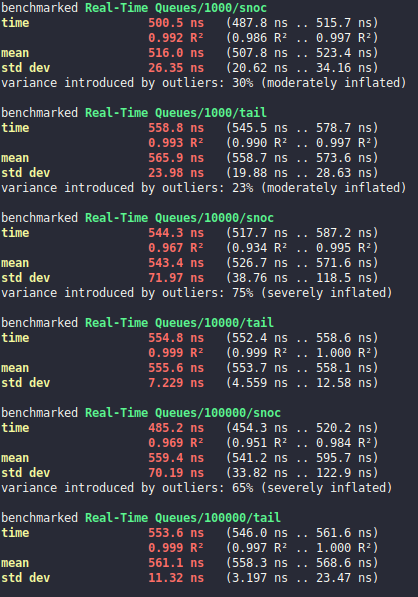
\includegraphics[scale=0.7]{experiment}
  \caption{Benchmarks results}
  \label{fig:experiment results}
\end{figure}

The results of the experiment appear in Figure \ref{fig:experiment results}.
The \textit{standard deviation} is low which is a good indicator that the values are near the mean of the set.
The \textit{real} execution time of these operations is inside the \textit{confidence interval}. As the range is narrow, we can assume that the values are significant.
Furthemore, the \textit{coefficient of determination} ($R^2$) is near $1$ which means that the observed outcomes replicate well the model with respect to the total variation.

\newpage

The results display similar \textit{mean} execution time for all operations independently of the size of the queue and the order of the operations.
Applying a \textit{Student's t-test} we can determine if all the operations do follow the same execution time.

From the previous results, we can conclude that the functional \textit{Real-Time Queues} from section \ref{ssub:Real-Time Queue} has a $O(1)$ worst-case running time.



%%%%%%%%%%%% Conclusion

\section{Conclusion}%
\label{sec:conclusion}

Reading \textit{Purely Functional Data Structures} has been very educative. The book is well structured and easy to follow. It has helped me to get a deeper understanding on how to design and implement purely functional data structures. And, I also learnt \textit{Standard M.L}, while reading the book, which is interesting from a programming language designer point of view.

Finally, it has helped me to get a better understanding of \textit{lazy evaluation} which, in conjunction with \textit{equational reasoning} and \textit{denotational semantics}, are still not very explored techniques.





%%%%%%%%%%%%%%%% BIBLIOGRAPHY %%%%%%%%%%%%%%%%%%%%%

\bibliographystyle{alpha}
\bibliography{refs}

\end{document}
